\section*{\textbf{1 - Normally distributed pseudo-random numbers} \hrule} 



\subsection*{\textbf{Question 1.a}}
\begin{quote}

\textbf{Problem}
\begin{quote}Write a random number generator that returns a random floating-point number between 0 and 1. At minimum, use some combination of an MWC and a 64-bit XOR-shift. Plot a sequential of random numbers against each other in a scatter plot ($x_{i+1}$ vs $x_{i}$) for the first 1000 numbers generated. Also plot the value of the random numbers for the first 1000 numbers vs the index of the random number, this mean the x-axis has a value from 0 through 999 and the y-axis 0 through 1). Finally, have your code generate 1,000,000 random numbers and plot the result of binning these in 20 bins 0.05 wide. 
\end{quote}

\textbf{Solution} 


\begin{quote}
The state of the random number generator is updated by first performing a 64-bit XOR-shift on the current state and then giving a modified version of the obtained output to the MWC algorithm. The modification of the XOR-shifts output consists of putting the last 32 bits to zero. This is done by performing the 'AND' operation with the maximum value of an unsigned int 32. This modification was performed as the  MWC algorithm expects as input a 64-bit unsigned integer with a value between  $0 < x < 2^{32}$.

The output of the MWC algorithm for this modified value is set as new state of the random number generator. The first 32 bits of the new state are used to provide a random value, as the output of the MWC algorithm only contains 32 significant bits. This random value is obtained by performing the 'AND' operation between the seed and the maximum value of an unsigned int 32. The resulting value is then divided by the maximum value of an uint32 to obtain a value between 0 and 1.

The code for the random number generator can be found at the end of this section, as it is treated as a shared module. The code for generating the plots and the created plots can be found below. 
\end{quote}
\newpage

\textbf{Code - Plots}


% consists of the code that initializes the random number generator and calls the function.

\begin{quote}
The code for generating the plots. The initialization of the created random number generator is not explicitly shown in this piece of code but can be found on page .. where the full code is shown that contains all sub-questions together.

\lstinputlisting[firstline=25,lastline=59]{./Code/assigment1.py}
\end{quote}
\end{quote}

\textbf{Code - Output text } 
\begin{quote}
The text output produced by the code:
\lstinputlisting[firstline=0,lastline=1]{./Output/assigment1_out.txt}
\end{quote}
\newpage

\textbf{Code - Output plots}
\begin{quote}

\begin{figure}[!ht]
\centering
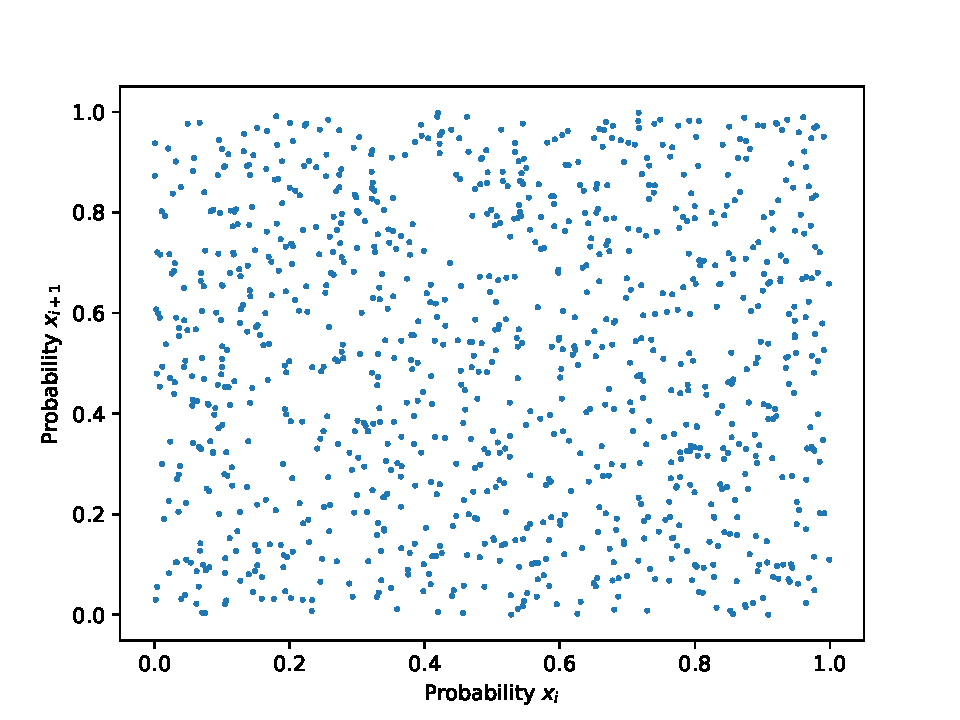
\includegraphics[width=12cm, height=7.5cm]{./Plots/1_plot_against.pdf}
\caption{TODO}
\end{figure}

\begin{figure}[!hb]
\centering
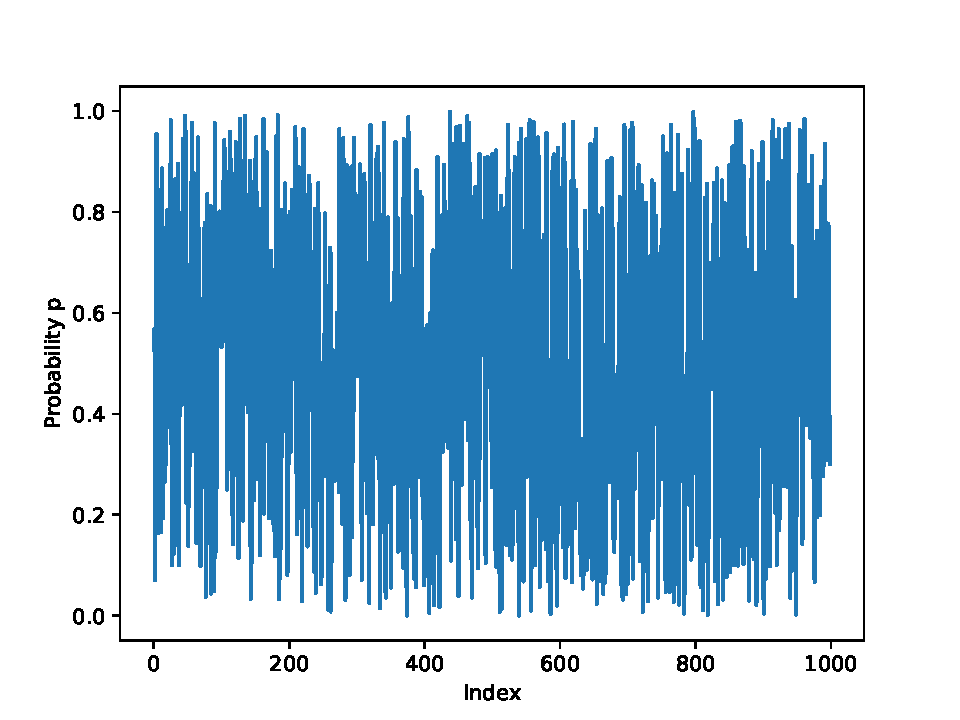
\includegraphics[width=12cm, height=7.5cm]{./Plots/1_plot_index.pdf}
\caption{TODO}
\end{figure}

\newpage
\begin{figure}[!ht]
\centering
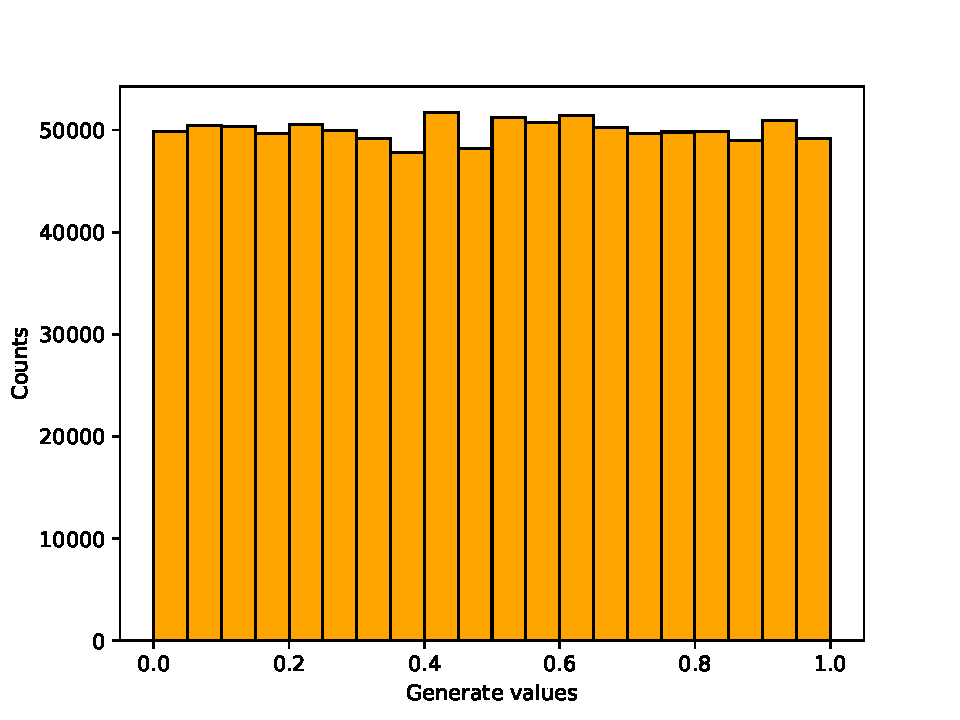
\includegraphics[width=12cm, height=7.5cm]{./Plots/1_hist_uniformnes.pdf}
\caption{TODO}
\end{figure}
\end{quote}


%\textbf{Code - helper } 
%\begin{quote}
%The code for the Poisson distribution and the factorial function.  
%\lstinputlisting[firstline=2,lastline=46]{./code/mathlib/utils.py}
%\end{quote}


%\textbf{Output}
%\begin{quote}
%The output produced by \textsf{/code/assigment1\_ a.py} 
%\lstinputlisting{./output/assigment1_a_out.txt}
%\end{quote}












